\documentclass[tikz,border=10pt]{standalone}
\usepackage{tkz-euclide} % 增强几何绘图功能
\begin{document}
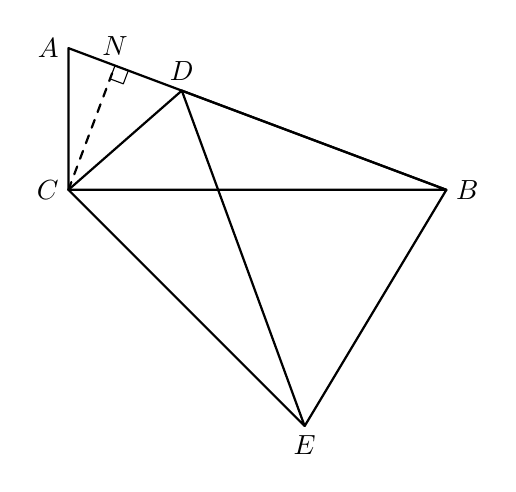
\begin{tikzpicture}[scale=1.2, line cap=round, line join=round]    
% 1. 定义核心顶点坐标 (根据图像比例估算)    
\coordinate (C) at (0,0);    
\coordinate (B) at (4,0);    
\coordinate (A) at (0,1.5);
    % 2. 构造 D 点 (在 AB 上) 与 E 点    
% 假设 D 在斜边 AB 上，E 是由某种旋转或对称关系确定的点    
\coordinate (D) at (0.8, 0.8*1.5/4 + 1.2); % 估算 D 点位置    
% 此处 D 点根据原图比例手动微调    
\coordinate (D) at (1.2, 1.05);    
\coordinate (E) at (2.5, -2.5); % E 点位于下方
    % 3. 绘制主要实线三角形和线段    
\draw[thick] (A) -- (B) -- (C) -- cycle; % 绘制三角形 ABC    
\draw[thick] (C) -- (D) -- (E) -- cycle; % 绘制三角形 CDE    
\draw[thick] (D) -- (B);     
\draw[thick] (E) -- (B);
    % 4. 辅助线：过 C 作 AB 的垂线点 N    
% 计算 C 到直线 AD (即直线 AB) 的垂足 N    
\coordinate (N) at ($(A)!(C)!(D)$);    
\draw[dashed, thick] (C) -- (N); % 垂线用虚线表示
    % 5. 标注直角符号 (点 N 处)    
\tkzMarkRightAngle[size=0.15](C,N,D)
    % 6. 标注顶点文字    
\node[left] at (A) {$A$};    
\node[left] at (C) {$C$};    
\node[right] at (B) {$B$};    
\node[above] at (D) {$D$};    
\node[below] at (E) {$E$};    
\node[above] at (N) {$N$};
    % 7. 细节微调：连接 DE 和 BD (已在循环和线段中完成)    
% 再次强调点的位置确保逻辑一致
\end{tikzpicture}
\end{document}